\documentclass[12pt, a4paper]{article}
\usepackage[italian]{babel}
\usepackage[margin=1.75cm]{geometry}
\usepackage{float}
\usepackage{graphicx}
\usepackage{hyperref}

\renewcommand{\familydefault}{\sfdefault}


\begin{document}
    \title{
        
\includegraphics[width=0.2\textwidth]{assets/logo.png}\\
        [0.5cm]CucinAssistant: Guida all'utilizzo\\
        \large aggiornata alla versione \emph{8 (Banana)}
    }
    \author{Gianluca Parri}
    \date{\today}
    \maketitle



    \tableofcontents
    \vfill
    \noindent Per segnalare errori o suggerimenti potete scrivere a
    \href{mailto:info@cucinassistant.com}{\mbox{info@cucinassistant.com}}.



    \section{Novità}
    
    Dall'ultima versione (\emph{7, Ciliegia}) sono state apportate le seguenti
    modifiche:

    \begin{itemize}
        \item Struttura dei menù personalizzabile (\ref{menus})
        \item Cambiate tutte le icone
    \end{itemize}

    \begin{figure}[H]
        \centering
        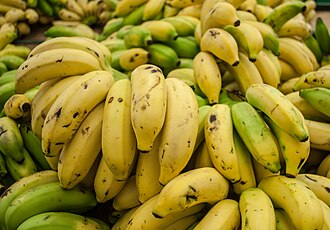
\includegraphics[width=0.45\textwidth]{assets/banane.jpg}
		\caption{\emph{Banane}. Foto da \href{https://commons.wikimedia.org/wi\
                ki/File:Cavendish_banana_from_Maracaibo.jpg}{qui}.}
    \end{figure}


    \section{Introduzione}

    \subsection{Cambio lingua}

    È possibile cambiare la lingua di visualizzazione in ogni momento cliccando
    il tasto apposito sulla barra di navigazione in alto.

    \begin{figure}[H]
        \centering
        
\includegraphics[width=0.45\textwidth]{assets/nav.png}
    \end{figure}

    \subsection{Registrazione e accesso}

    Se avete già un account potete inserire le vostre credenziali nella pagina
    di accesso; altrimenti potete cliccare il pulsante \emph{Registrati} per
    crearne uno nuovo.

    Nel caso aveste dimenticato il nome utente e/o la password, cliccando il
    tasto \emph{Password dimenticata}, vi verrà inviata una email contenente il
    nome utente e un link per cambiare la password.

    \begin{figure}[H]
        \centering
        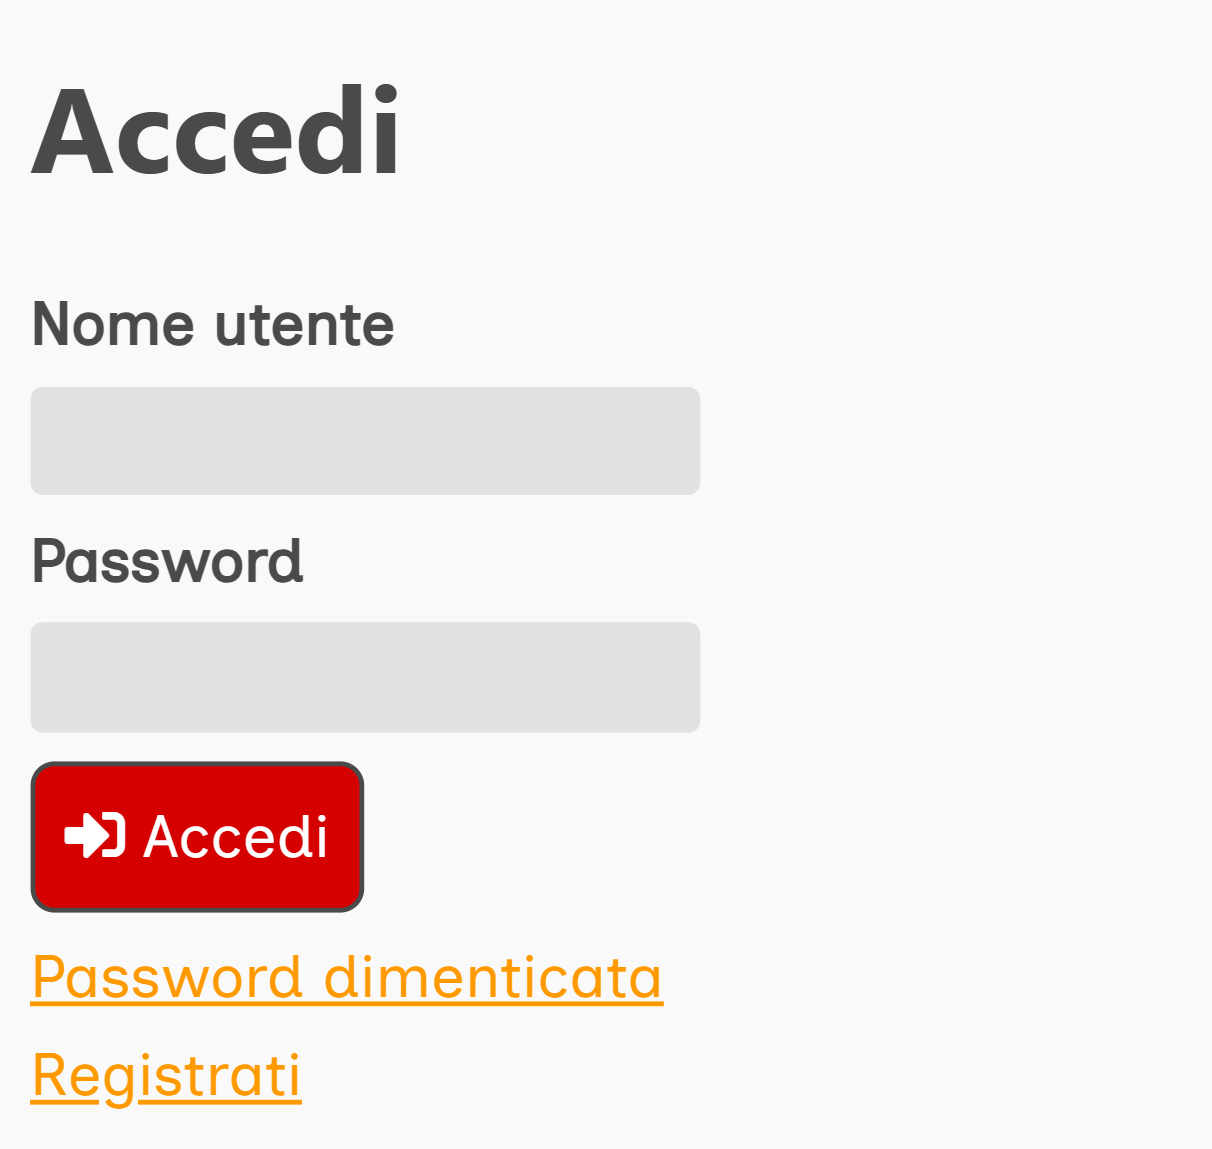
\includegraphics[width=0.45\textwidth]{assets/it/signin.png}
    \end{figure}

    Una volta entrati, avrete accesso alla \emph{homepage}.

    \begin{figure}[H]
        \centering
        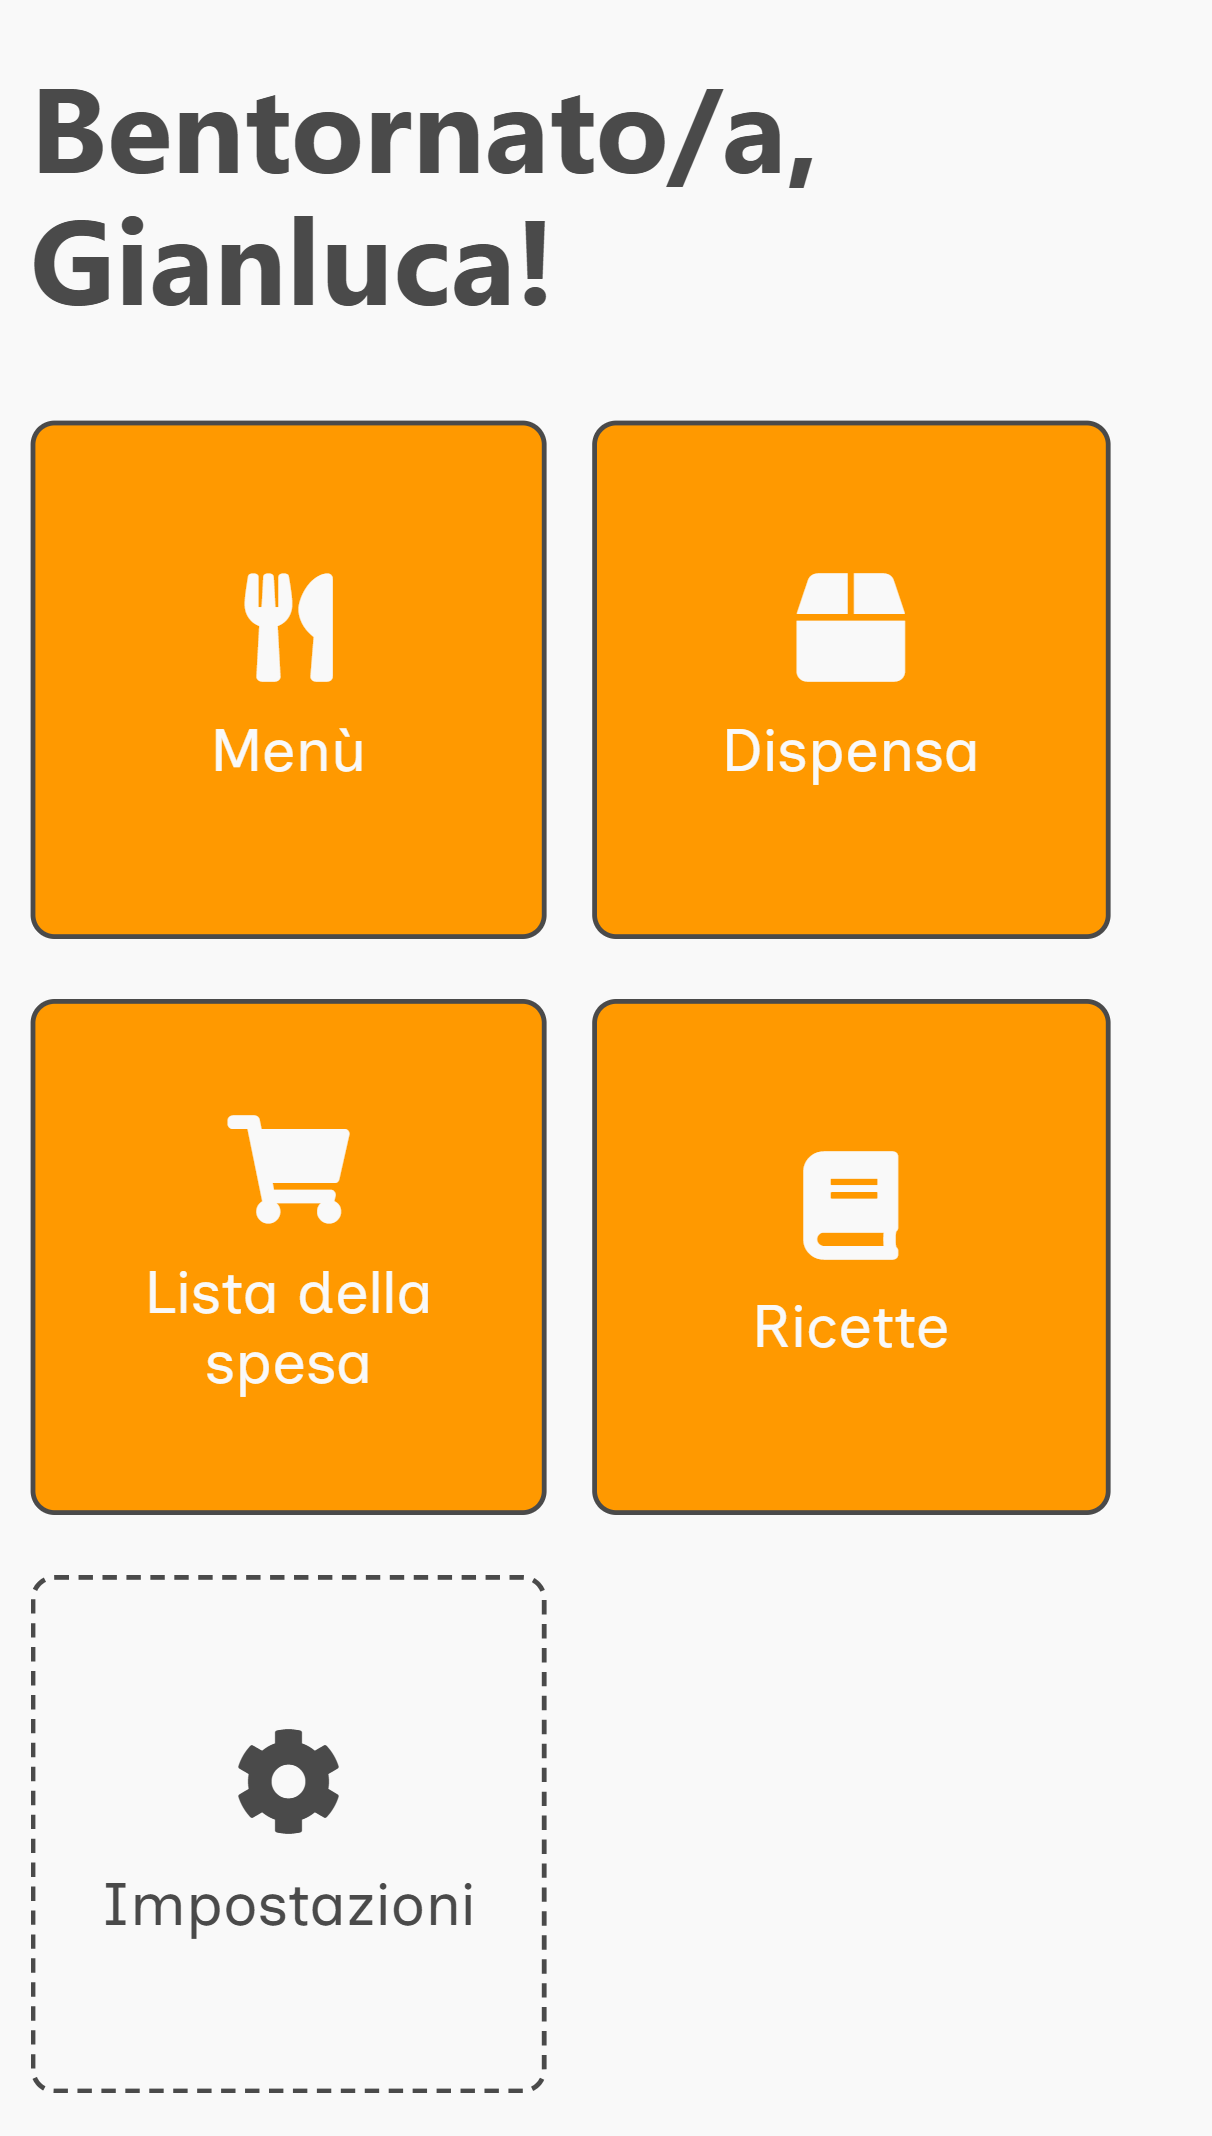
\includegraphics[width=0.45\textwidth]{assets/it/home.png}
    \end{figure}

    \subsection{Impostazioni}

    Dalle impostazioni è possibile disconnettersi, cambiare i dati personali
    (nome utente, email, password), le preferenze sulle email
    (lingua e consenso alla newsletter) ed eliminare definitivamente l'account.

    \begin{figure}[H]
        \centering
        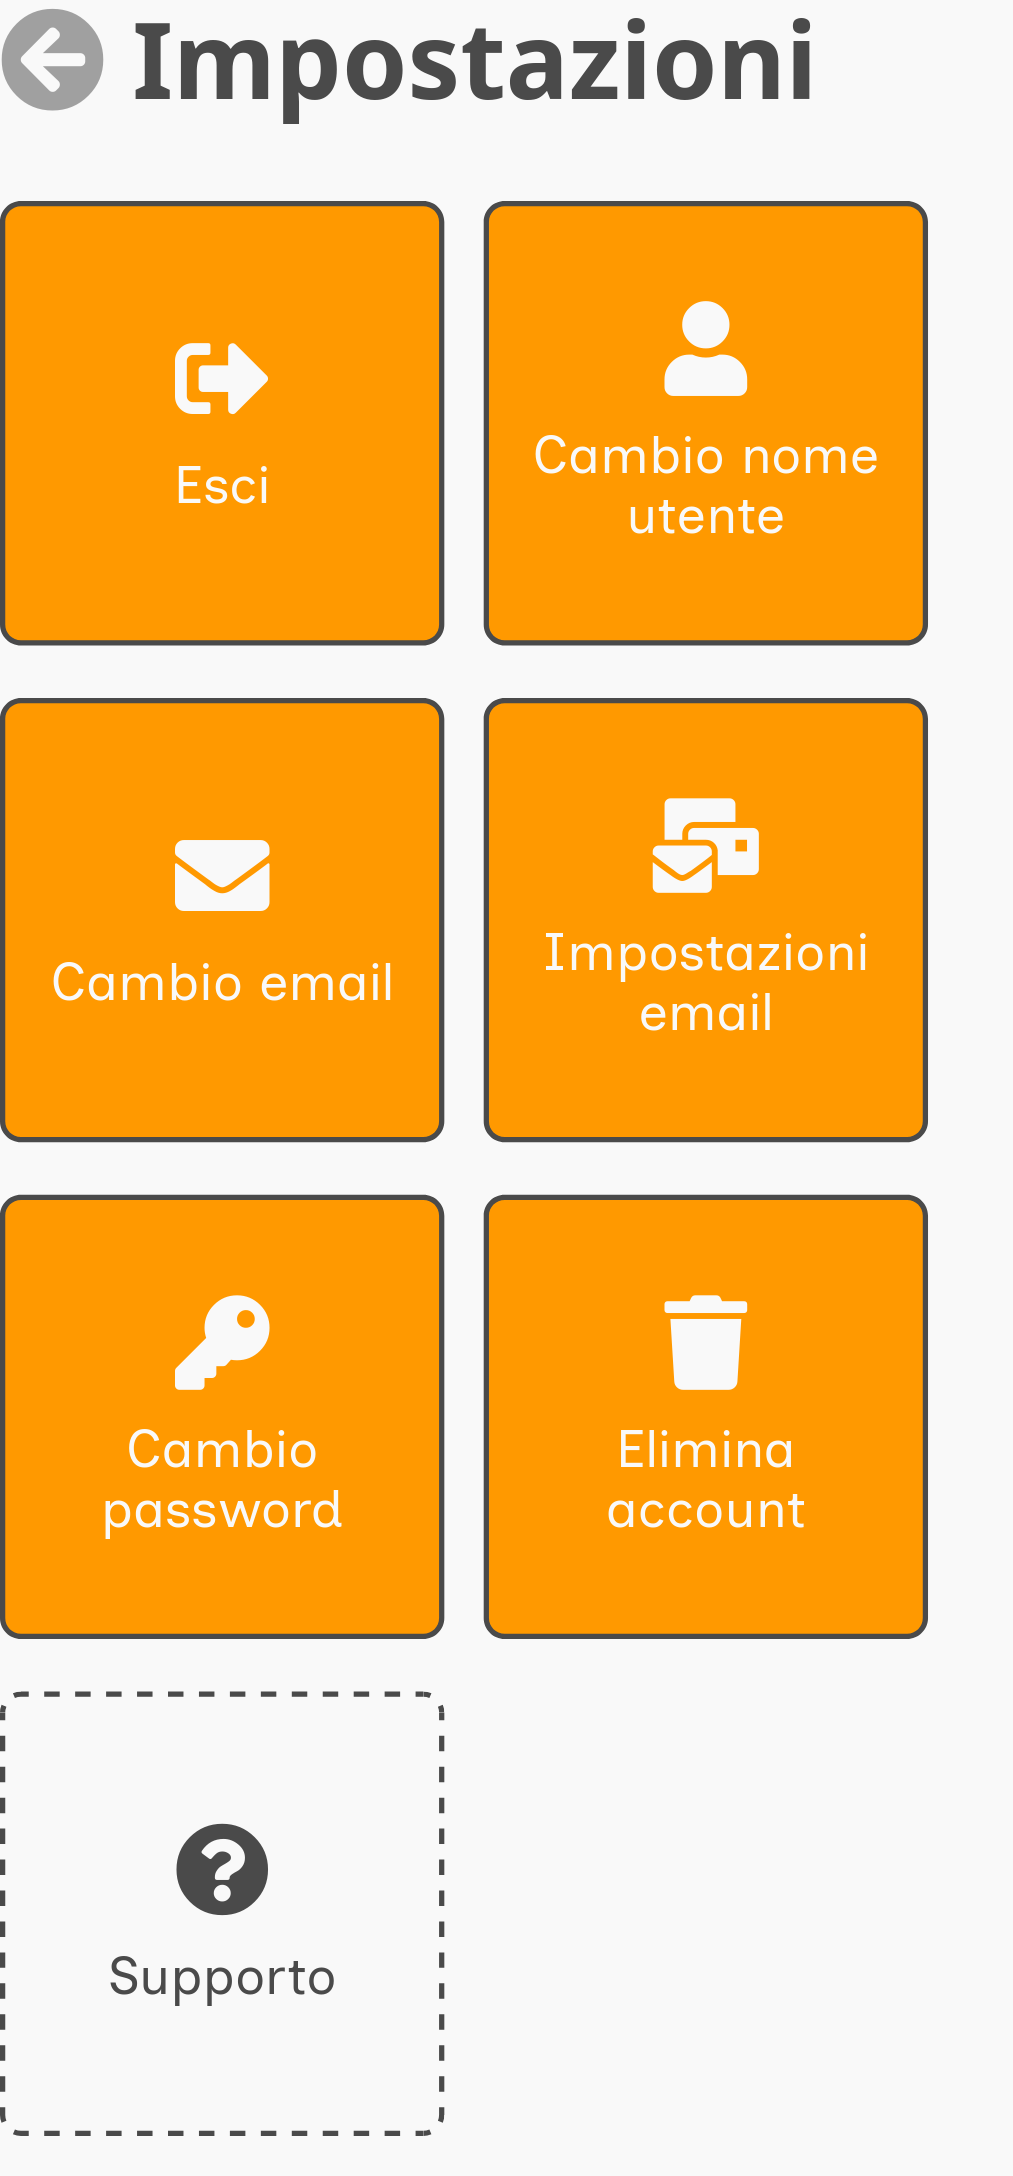
\includegraphics[width=0.45\textwidth]{assets/it/settings.png}
    \end{figure}


    \section{Menù} \label{menus}

    \subsection{Creazione}

    Cliccando il tasto apposito è possibile creare un nuovo menù, specificando
    i giorni inclusi e il numero di pasti per ogni giorno (poi modificabile in)
    seguito.

    \begin{figure}[H]
        \centering
        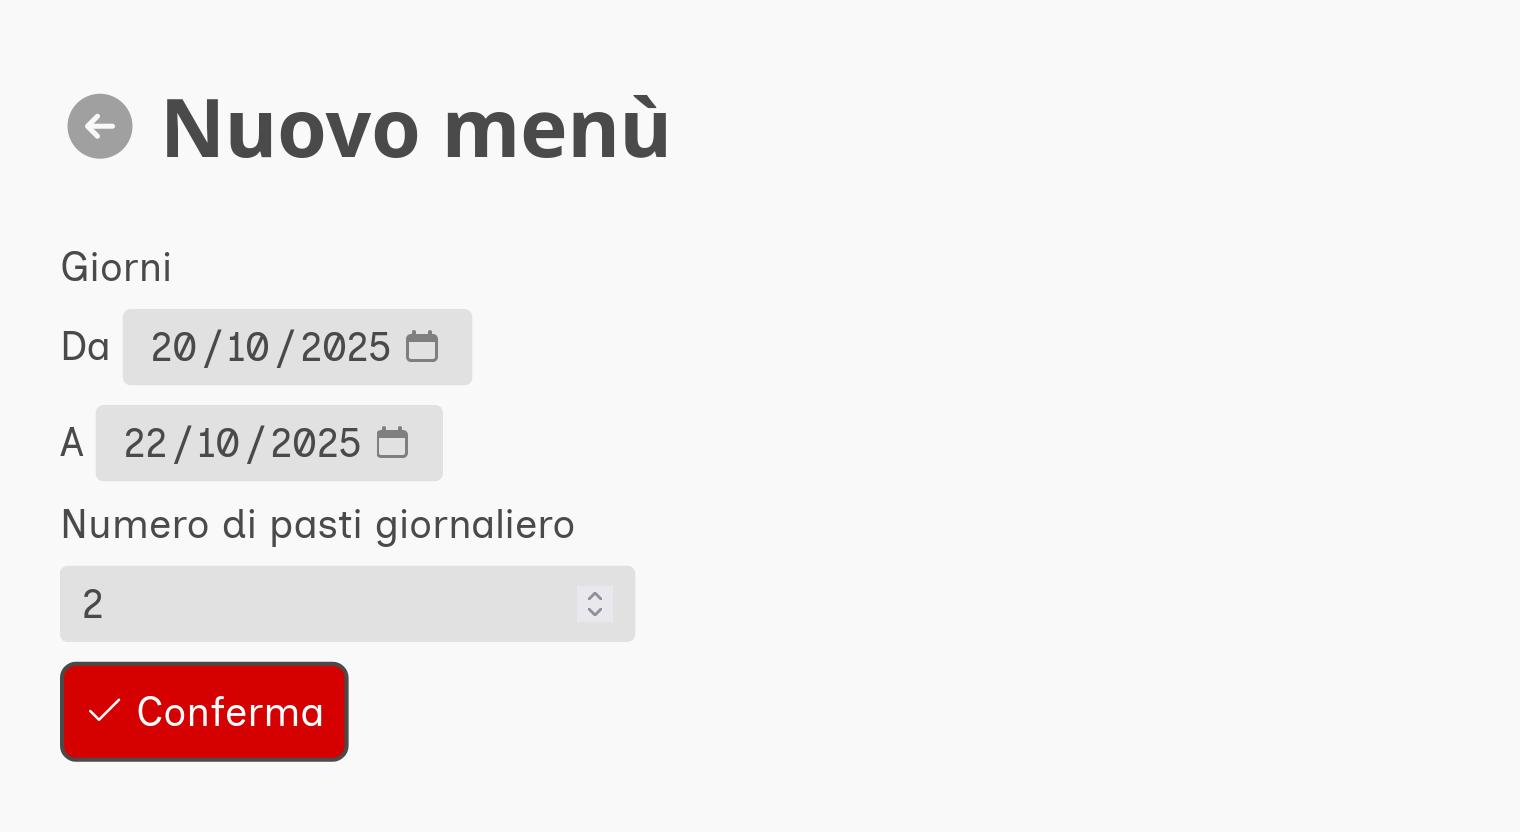
\includegraphics[width=0.45\textwidth]{assets/it/menu_new.png}
    \end{figure}

    \subsection{Modifica}

    Per modificare il contenuto del menù è sufficiente cliccare il tasto
    \emph{Modifica}.
    
    Dalla pagina che si aprirà sarà possibile modificare il nome del menù o
    eliminarlo; inoltre, saranno presenti una serie di pulsanti che
    permetteranno di modificare giorno per giorno.

    \begin{figure}[H]
        \centering
        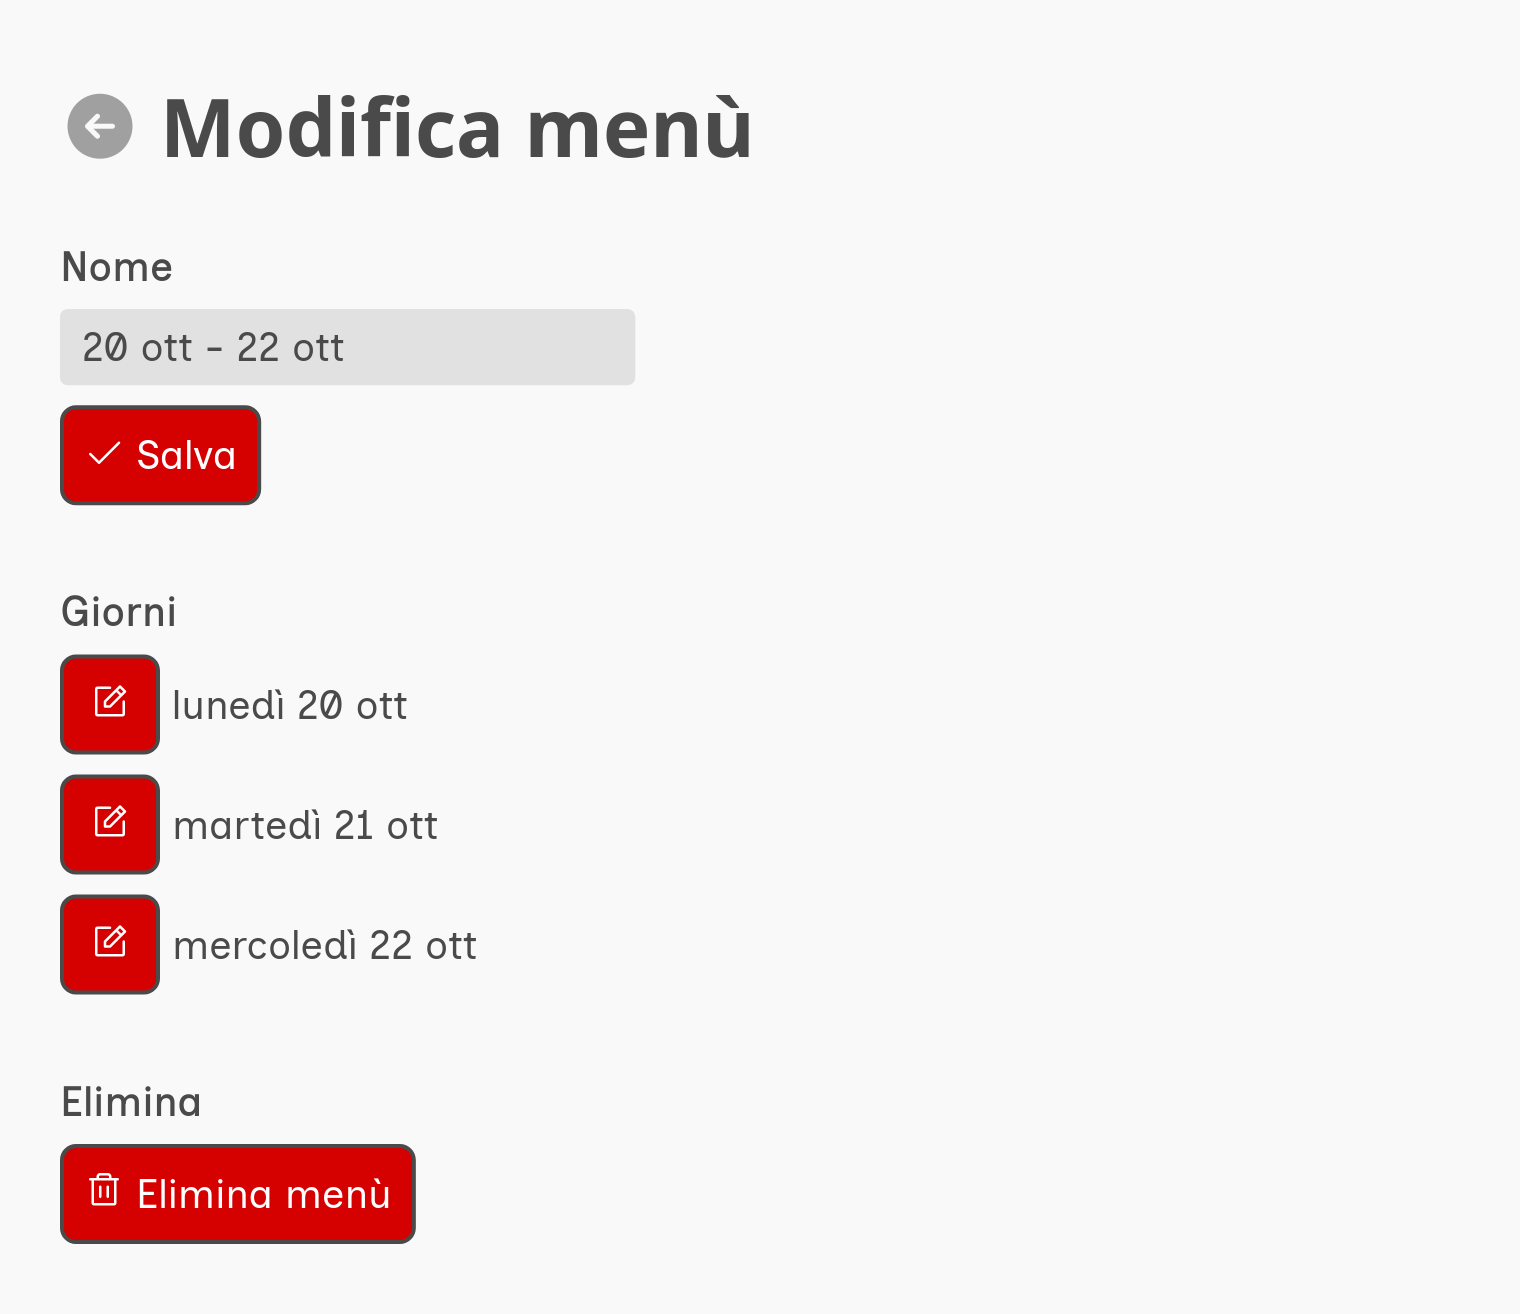
\includegraphics[width=0.45\textwidth]{assets/it/menu_edit.png}
    \end{figure}

    Nella pagina di modifica del giorno è possibile cambiarne il nome o i
    pasti, aggiungendoli o eliminandoli all'occorrenza.

    \begin{figure}[H]
        \centering
        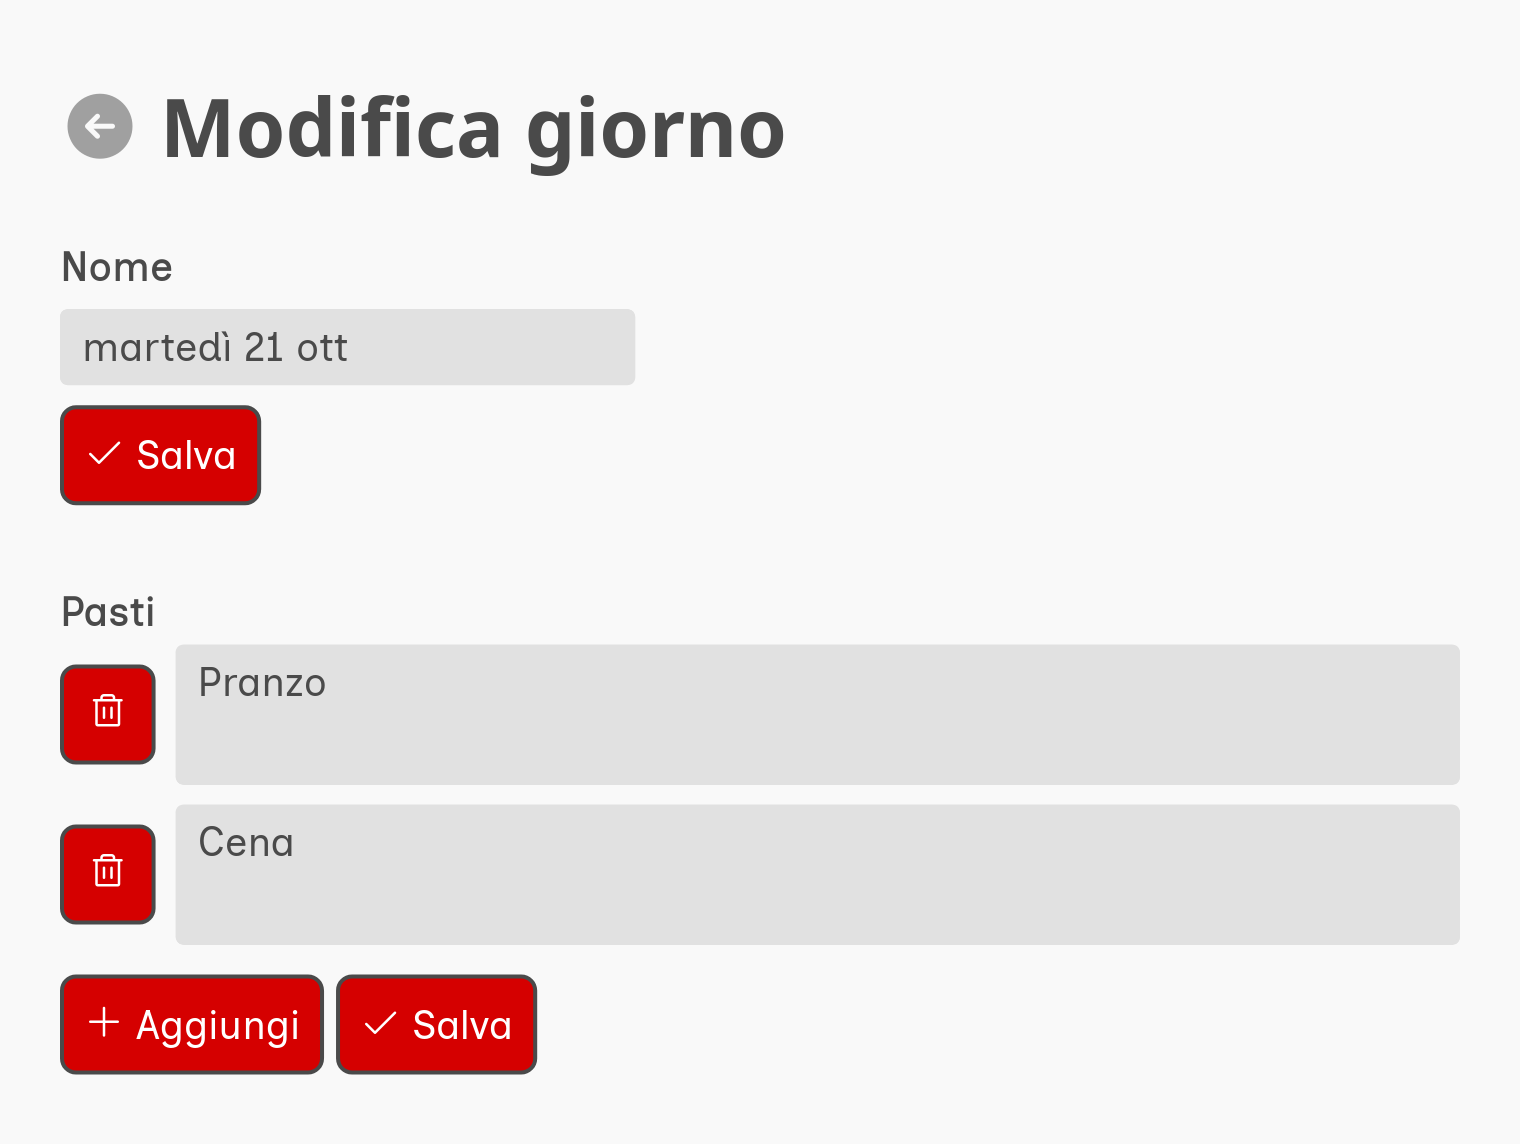
\includegraphics[width=0.45\textwidth]{assets/it/menu_day.png}
    \end{figure}



    \section{Dispensa}

    All'interno della dispensa potete inserire degli articoli con un nome, una
    data di scadenza (opzionale) e una quantità (intera o decimale; opzionale).

	\subsection{Sezioni}

    Gli articoli saranno raggruppati in sezioni, visibili all'apertura della
    \emph{Dispensa}.

    \begin{figure}[H]
        \centering
        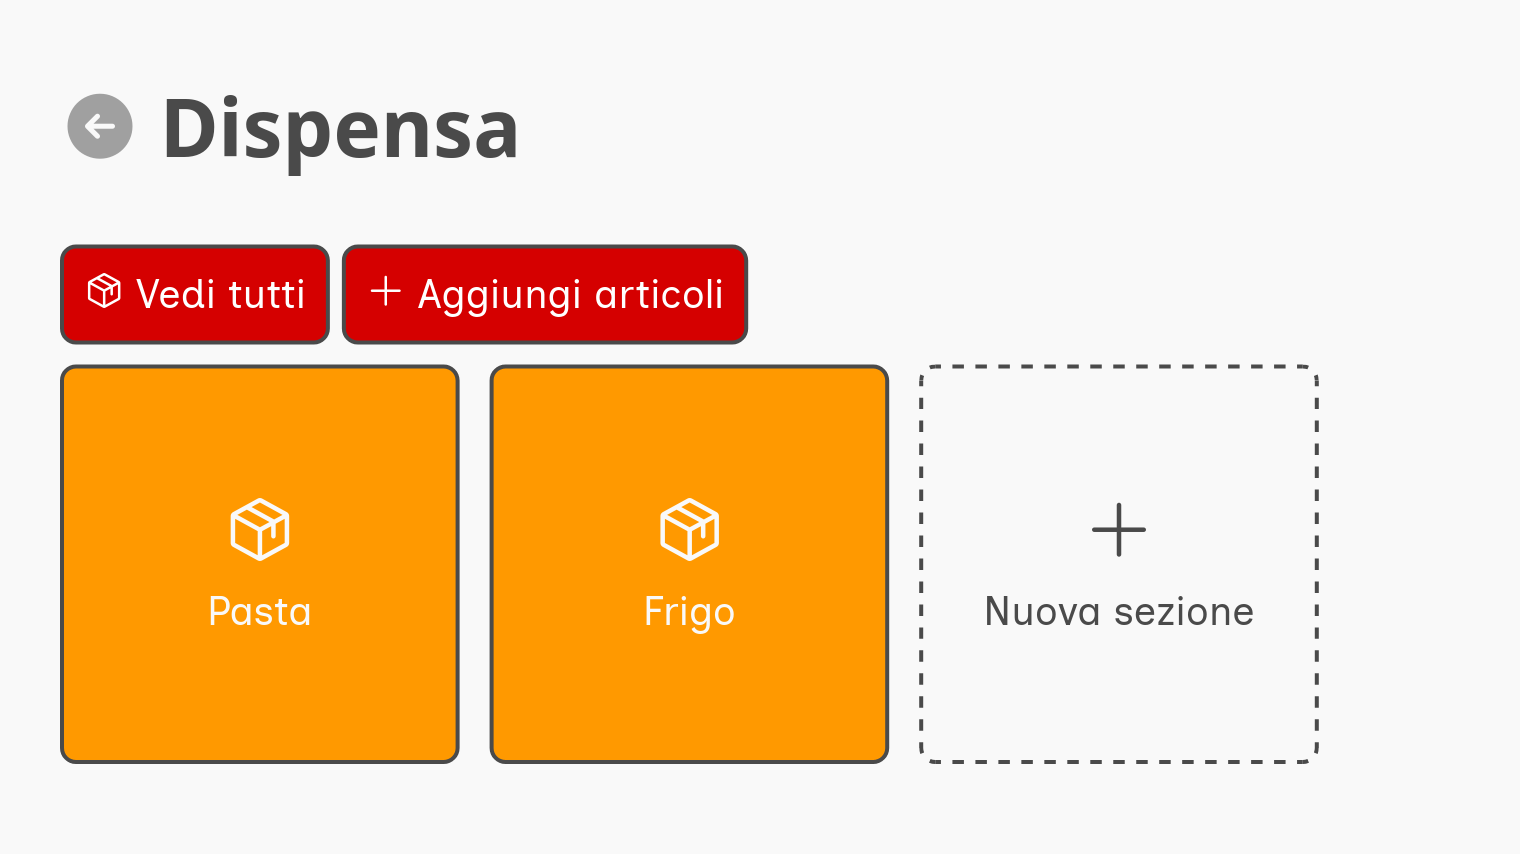
\includegraphics[width=0.45\textwidth]{assets/it/storage.png}
    \end{figure}

    Potete creare nuove sezioni con il pulsante apposito; per modificarne
    o eliminarne una sarà necessario aprirla e cliccare sul pulsante
    \emph{Modifica sezione}.

    \subsection{Articoli}

	Per vedere gli articoli (di una sezione, o tutti in generale) basterà
    cliccare il pulsante apposito. Se necessario, è possibile fare una ricerca
	per nome.

    Gli articoli sono ordinati in base alla loro data di scadenza; quelli
    scaduti sono contrassegnati da una banda laterale rossa al posto di quella
    arancione.

    \begin{figure}[H]
        \centering
        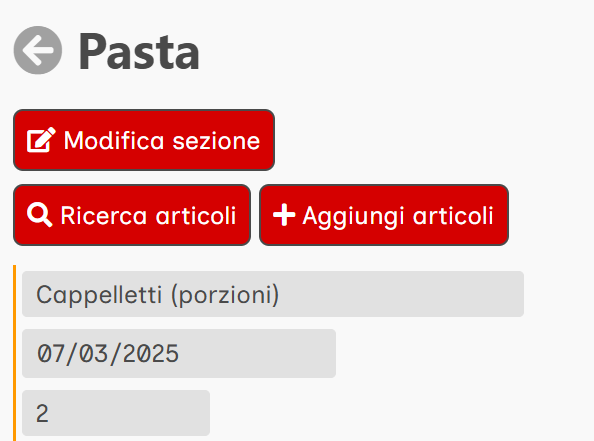
\includegraphics[width=0.45\textwidth]{assets/it/articles.png}
    \end{figure}

    È possibile aggiungere articoli sia dall'interno di una sezione che dalla
    pagina principale: in questo caso, per ogni articolo è necessario
    specificare la sezione in cui deve essere salvato.

    Un articolo è identificato dal nome e dalla data di scadenza, quindi se
    verrà inserito un articolo con stesso nome e data di scadenza di uno già in
    dispensa, non verranno creati duplicati, ma le quantità verranno sommate.

    \subsection{Modifica di articoli}

    Cliccando su un articolo, questo verrà aperto e mostrato con due frecce
    (per scorrere tra gli articoli) e un bottone \emph{Elimina}.

    Una volta cambiati dei dati, i pulsanti precedenti verranno sostituiti da
    \emph{Salva} e \emph{Annulla}, per confermare le modifiche effettuate.
    Cambiando la sezione l'articolo verrà spostato.
    
    Cambiando la data di scadenza di un articolo è possibile che l'ordine
    cambi: in questo caso si tornerà alla visualizzazione a lista.

    \begin{figure}[H]
        \centering
        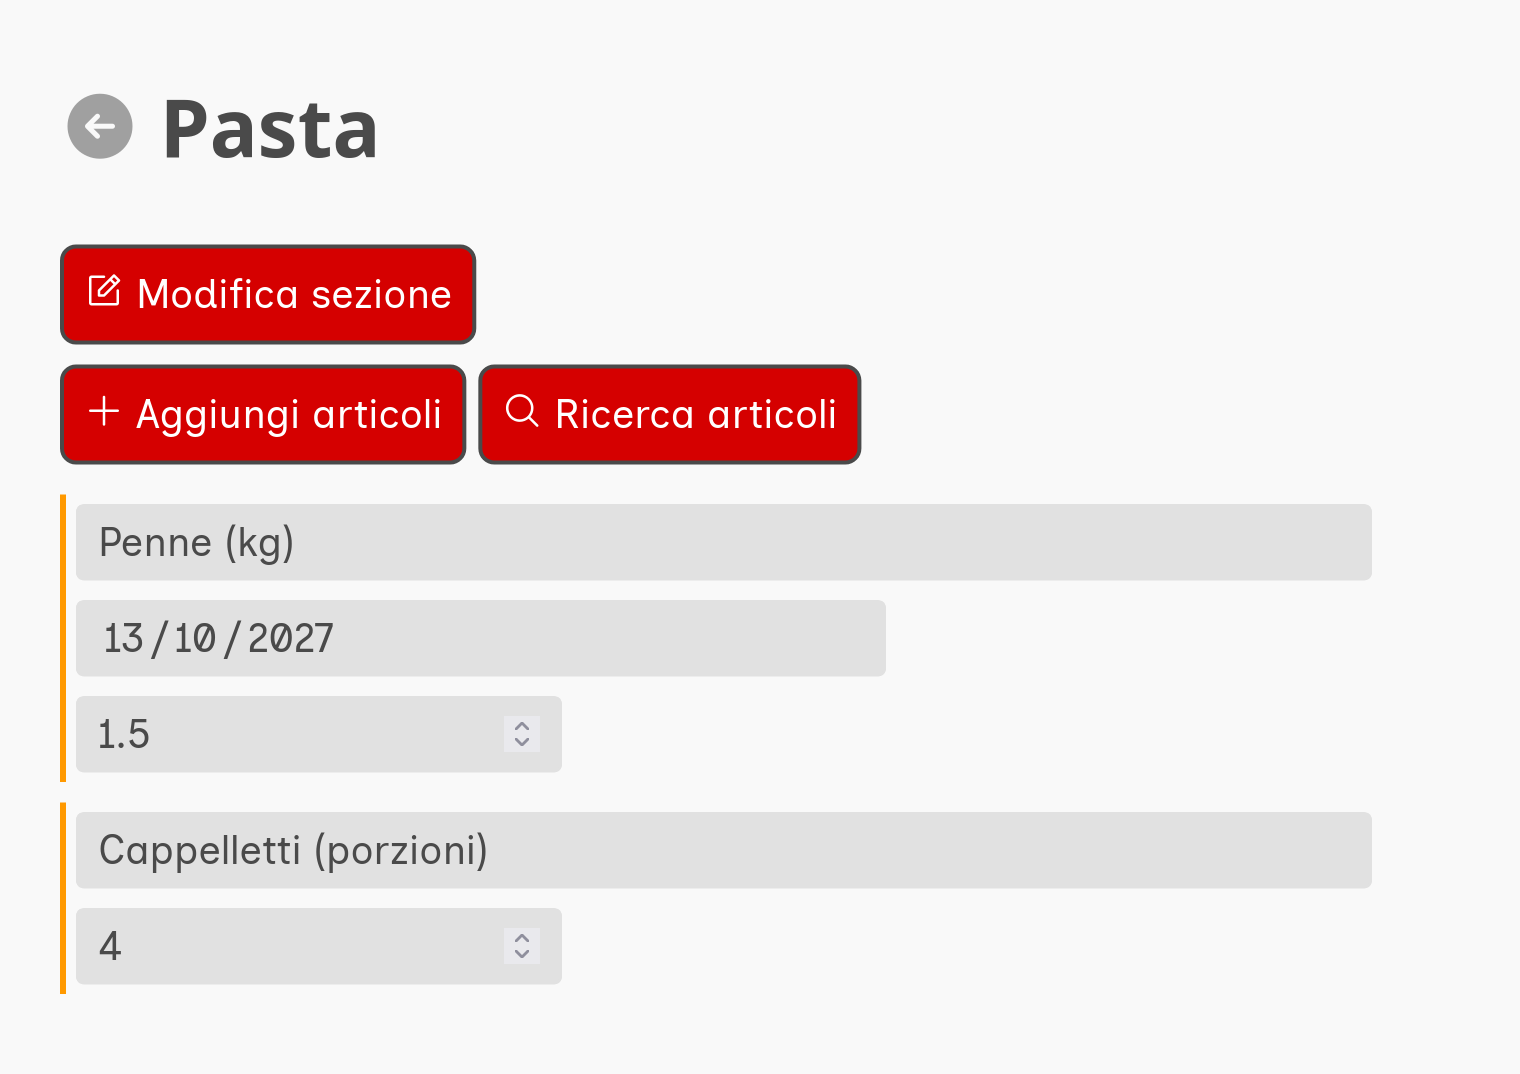
\includegraphics[width=0.45\textwidth]{assets/it/article.png}
    \end{figure}



    \section{Lista della spesa}

    \subsection{Panoramica}

    È... una lista della spesa.

    \begin{figure}[H]
        \centering
        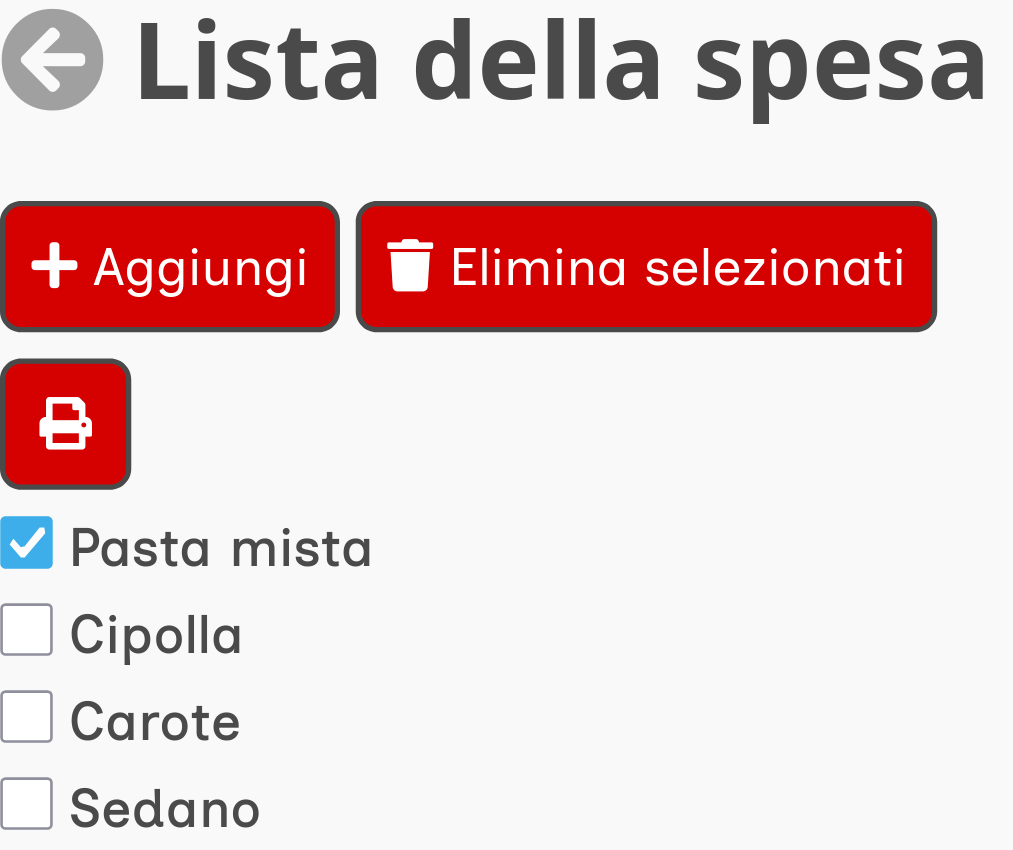
\includegraphics[width=0.45\textwidth]{assets/it/shopping_list.png}
    \end{figure}

    Cliccando sul quadrato a sinistra del nome di un elemento, questo verrà
    spuntato, ma rimarrà in lista; per eliminare tutti gli elementi spuntati
    basterà cliccare il tasto apposito.

    Per aggiungere nuovi elementi potete usare il pulsante \emph{Aggiungi}; per
    modificarne uno basterà cliccare sul nome.



    \section{Ricette}

    Una ricetta è composta da un nome (l'unica componente obbligatorio), una
    valutazione (da 0,5 a 5,0 stelle), una lista di ingredienti, un
    procedimento e delle note aggiuntive.

    \subsection{Panoramica}

    Cliccando il pulsante \emph{Ricette} potrete vedere tutte le ricette
    salvate, e un bottone per crearne di nuove.

    \begin{figure}[H]
        \centering
        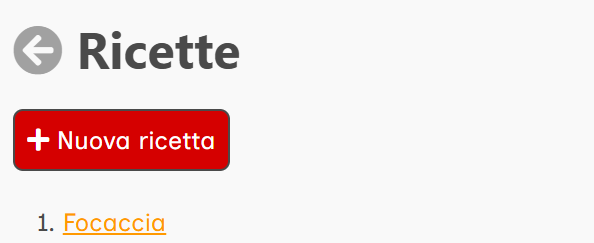
\includegraphics[width=0.45\textwidth]{assets/it/recipes.png}
    \end{figure}

    Per vederne una in dettaglio basterà cliccarla.

    \begin{figure}[H]
        \centering
        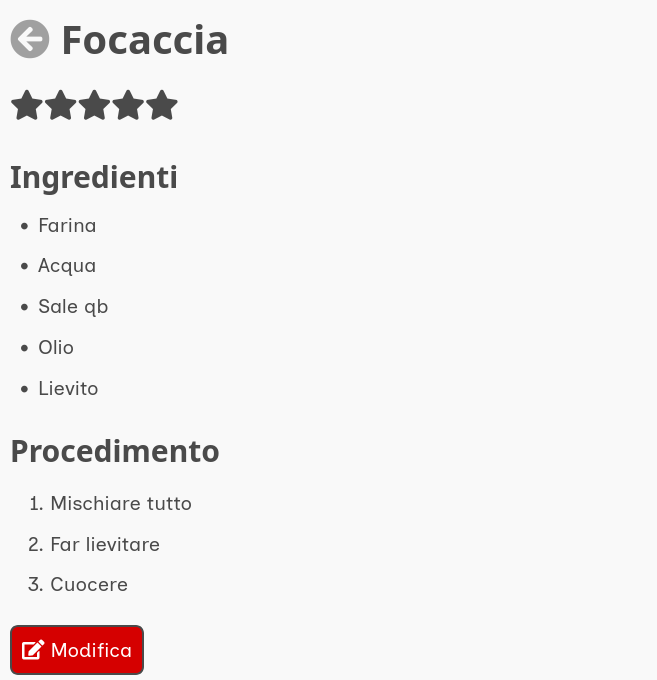
\includegraphics[width=0.45\textwidth]{assets/it/recipe.png}
    \end{figure}

    Per modificarla o eliminarla potete cliccare sul pulsante \emph{Modifica}.

    Per una formattazione corretta, è importante ricordarsi di andare a capo
    durante la scrittura degli ingredienti e del procedimento.

    Per nascondere le stelle potete impostarne il numero a 0.

	\subsection{Condivisione}

	Nel caso in cui vogliate condividere una ricetta, cliccando il tasto
    \emph{Condividi}, sarà possibile sia ottenerne una versione pdf, sia
    generare un link di condivisione (poi revocabile in seguito), tramite il
    quale sarà possibile accedere alla ricetta. Se condivisa tramite link, ogni
    modifica fatta alla ricetta sarà visibile anche a tutti coloro che hanno il
    link.

    \begin{figure}[H]
        \centering
        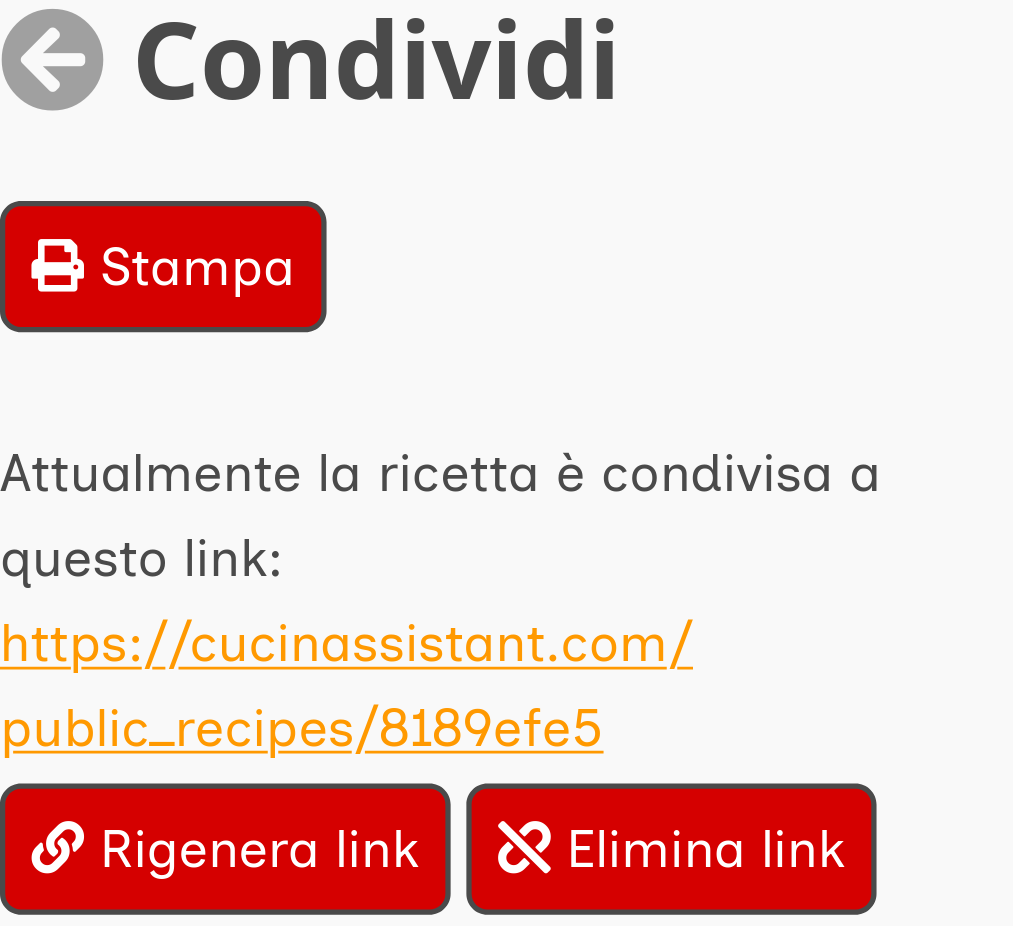
\includegraphics[width=0.45\textwidth]{assets/it/recipe_sharing.png}
    \end{figure}

	Gli utenti registrati possono salvare nel loro account una copia di una
    ricetta condivisa tramite link; in questo caso le modifiche non saranno
    sincronizzate, ma la copia rimarrà anche nel caso il link venga revocato.
\end{document}
